% !TeX spellcheck = en_US
\documentclass[french]{yLectureNote}

\title{Atomistique}
\subtitle{La matière à l'échelle atomique}
\author{Paulhenry Saux}
\date{\today}
\yLanguage{Français}

\professor{J.Cuny}%sebastien.deveuhels.irap.omp.eu

\usepackage{graphicx}%----pour mettre des images
\usepackage[utf8]{inputenc}%---encodage
\usepackage{geometry}%---pour modifier les tailles et mettre a4paper
%\usepackage{awesomebox}%---pour les boites d'exercices, de pbq et de croquis ---d\'esactiv\'e pour les TP de PC
\usepackage{tikz}%---pour deiffner + d\'ependance de chemfig
\usepackage{tkz-tab}
\usepackage{chemfig}%---pour deiffner formules chimiques
\usepackage{chemformula}%---pour les formules chimiques en \'equation : \ch{...}
\usepackage{tabularx}%---pour dimensionner automatiquement les tableaux avec variable X
\usepackage{awesomebox}%---Pour les boites info, danger et autres
\usepackage{menukeys}%---Pour deiffner les touches de Calculatrice
\usepackage{fancyhdr}%---pour les en-t\^ete personnalis\'ees
\usepackage{blindtext}%---pour les liens
\usepackage{hyperref}%---pour les liens (\`a mettre en dernier)
\usepackage{caption}%---pour la francisation de la l\'egende table vers Tableau
\usepackage{pifont}
\usepackage{array}%---pour les tableaux
\usepackage{lipsum}
\usepackage{yFlatTable}
\usepackage{multicol}
\newcommand{\Lim}[1]{\lim\limits_{\substack{#1}}\:}
\renewcommand{\vec}{\overrightarrow}
\begin{document}
\setcounter{chapter}{3}
\chapter{Orbitales Atomiques hybridées et moléculaires}
\section{Hybridation d'OA et liaison}
\subsection{Hybridation}
Pour représenter les géométrie, on fait des combinaisons linéaires des OA. Les OA issues de ces dernières sont dites hybridées. Le nombre d'OA dans la combinaison dépend de la géométrie que l'on veut obtenir.

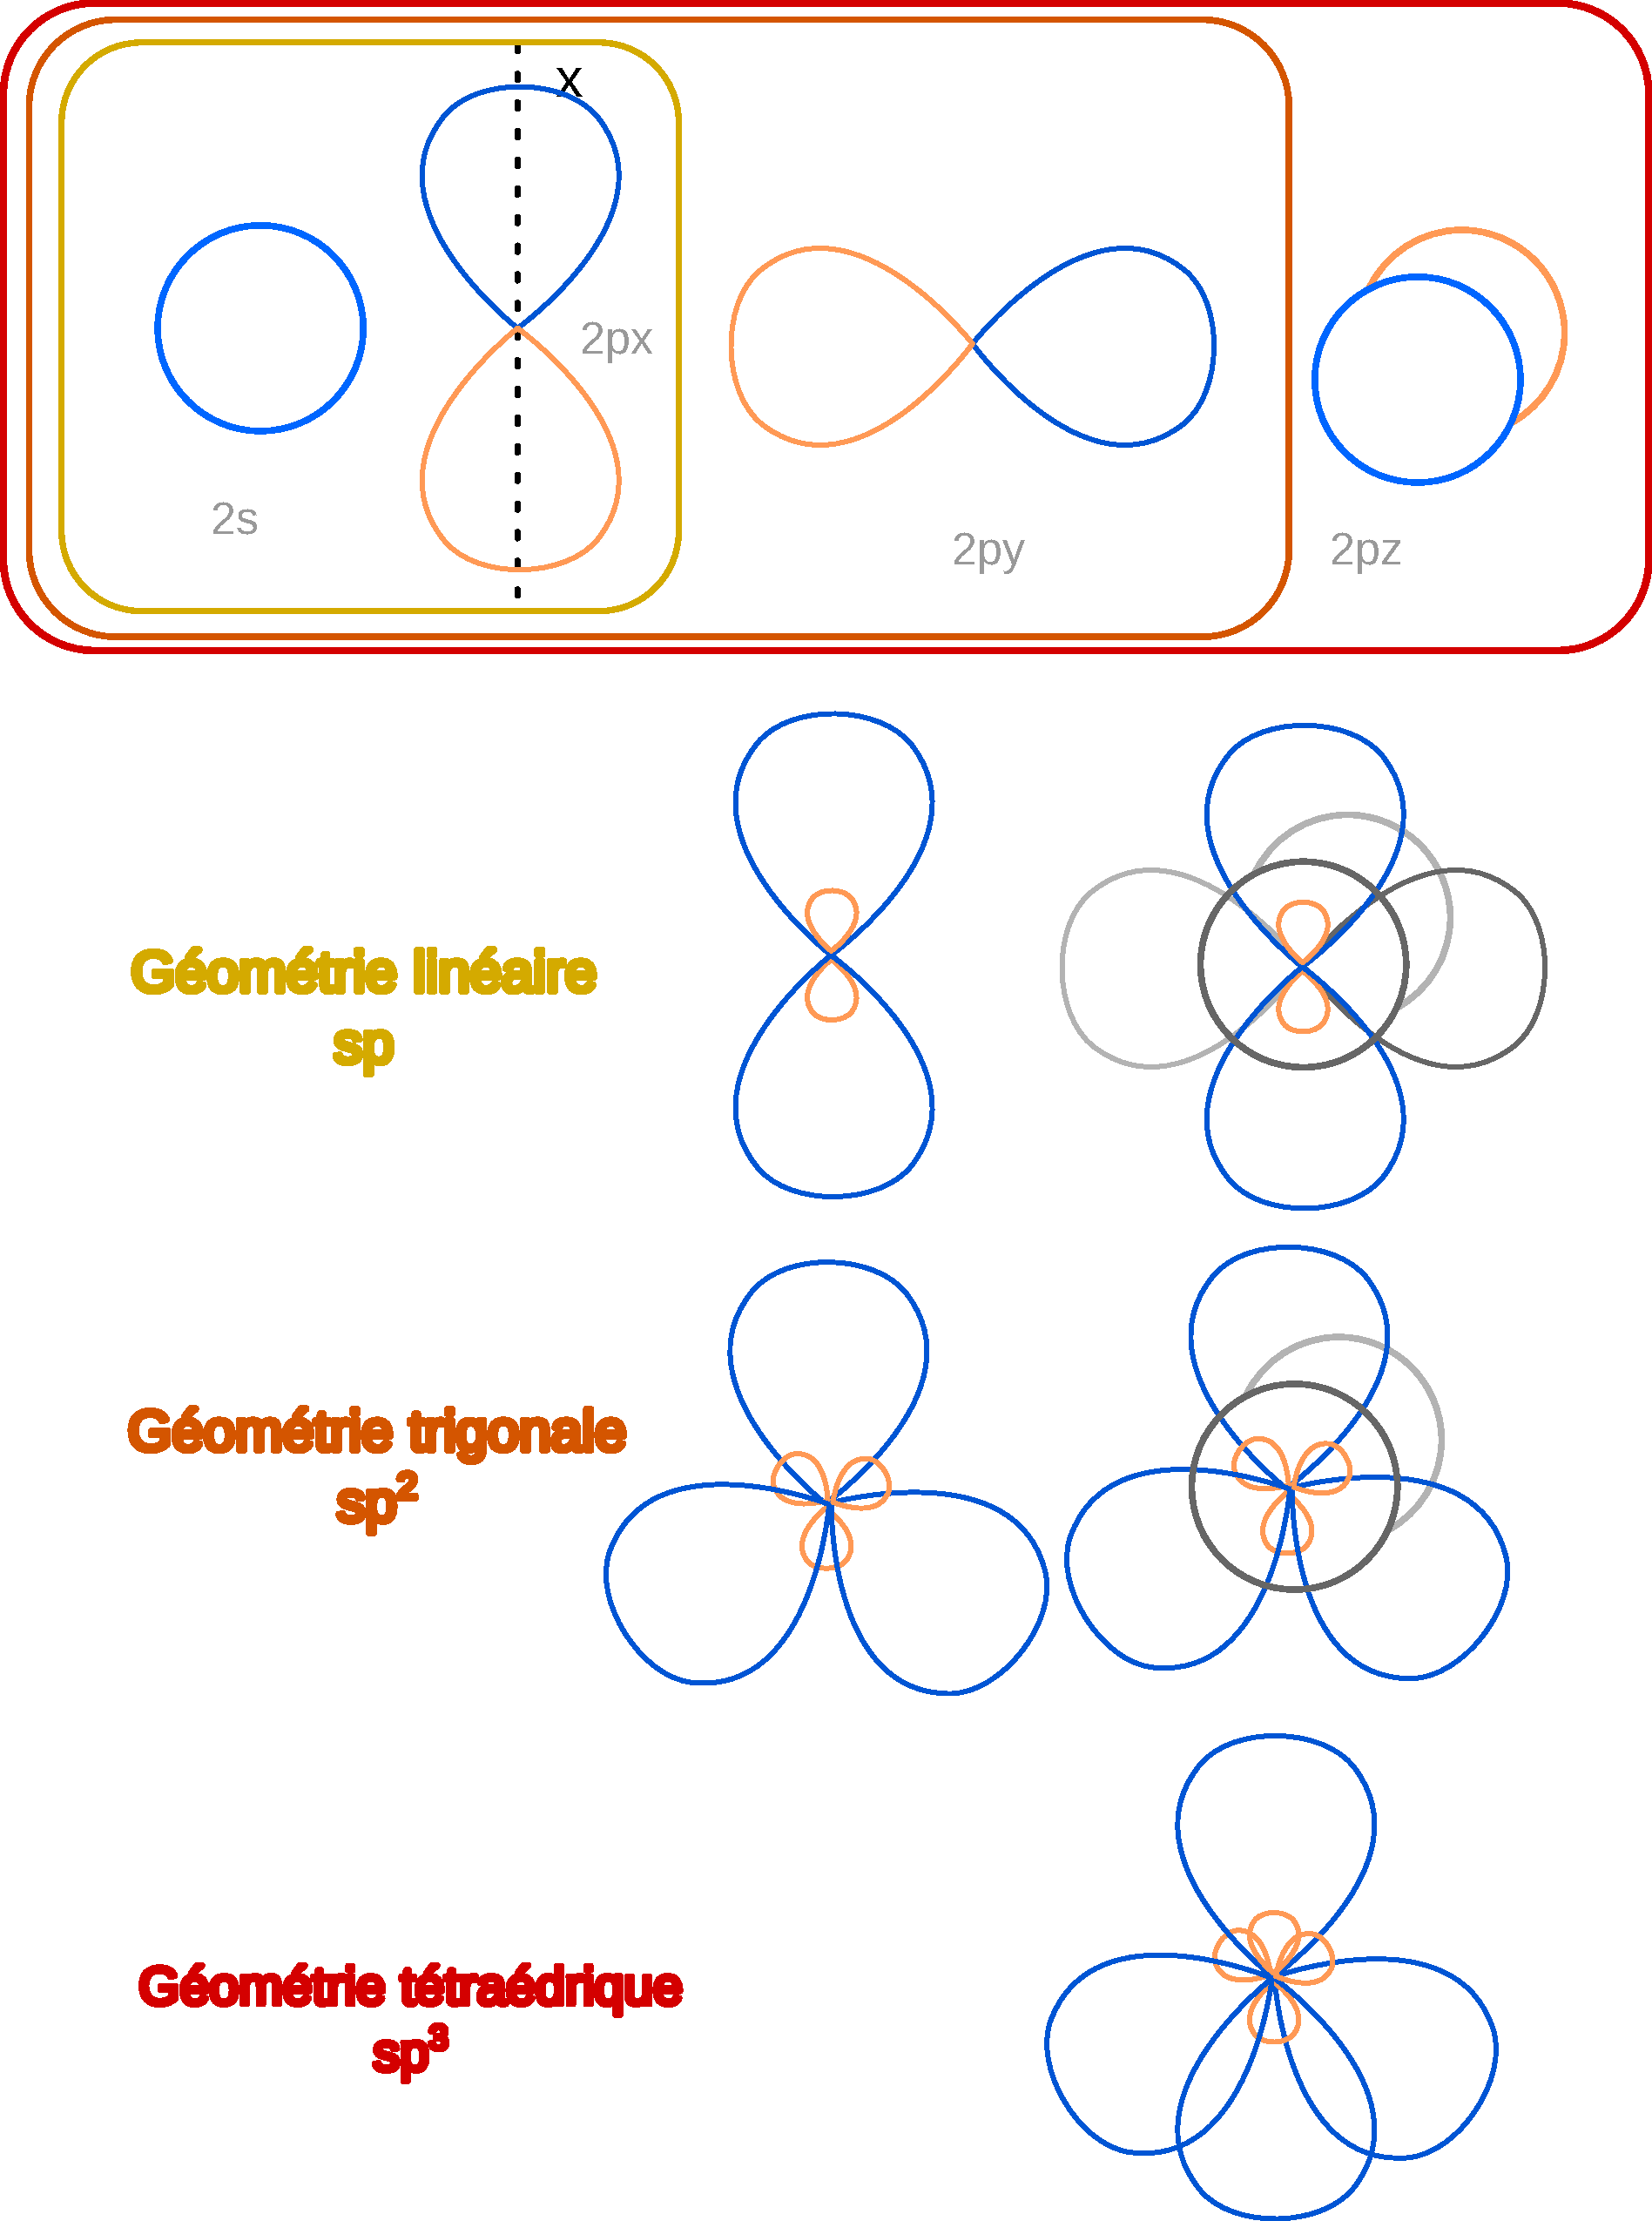
\includegraphics[scale=0.25]{hybridation}
\subsection{Liaisons}
On distingue 2 types de liaison :
\begin{itemize}
 \item Liaison $\sigma$ : Intéraction entre 2 OA avec une symétrie de révolution le long de l'axe de la liaison\marginInfo{L'OA ne change pas tout autour de l'axe}.
 \item Liaison $\pi$ : Intéraction entre 2 OA présentant un plan d'antisymétrie contenant l'axe de la liaison\marginInfo{Il s'agit d'un plan de symétrie mais avec un changement de signe des OA par la symétrie}. Elles sont d'une énergie plus faible que les liaisons $\sigma$ mais peuvent se délocaliser.\marginCritical{Ce sont les seules à pouvoir le faire. Les liaisons $\sigma$ ne le font pas ou extrêmement rarement.}
\end{itemize}
\warningInfo{Lien avec le type de liaison et l'hybridation}{
Les orbitales hybridées produisent des liaison $\sigma$ et celles non hybridées des liaisons $\pi$.}
Dans les molécules, les liaisons doubles sont constituées d'une liaison $\sigma$ et d'une $\pi$. Les triples  sont constituées d'une liaison $\sigma$ et de deux $\pi$.

\subsection{Représentation}
Une fois le schéma de Lewis effectué puis la représentation VSEPR, on détermine la figure de répulsion des atomes afin de déterminer le type d'hybridation des OA. Enfin, remplace dans le schéma VSEPR les atomes par leur OA.
\criticalInfo{Géométrie}{Pour déterminer le type d'hybridation, il faut prendre en compte la figure de répulsion de l'atome et non sa géométrie ou formule VSEPR. Par exemple, pour une formule $AX_2E$, on prend la figure $AX_3$, donc une géométrie trigonale, et non coudée.}
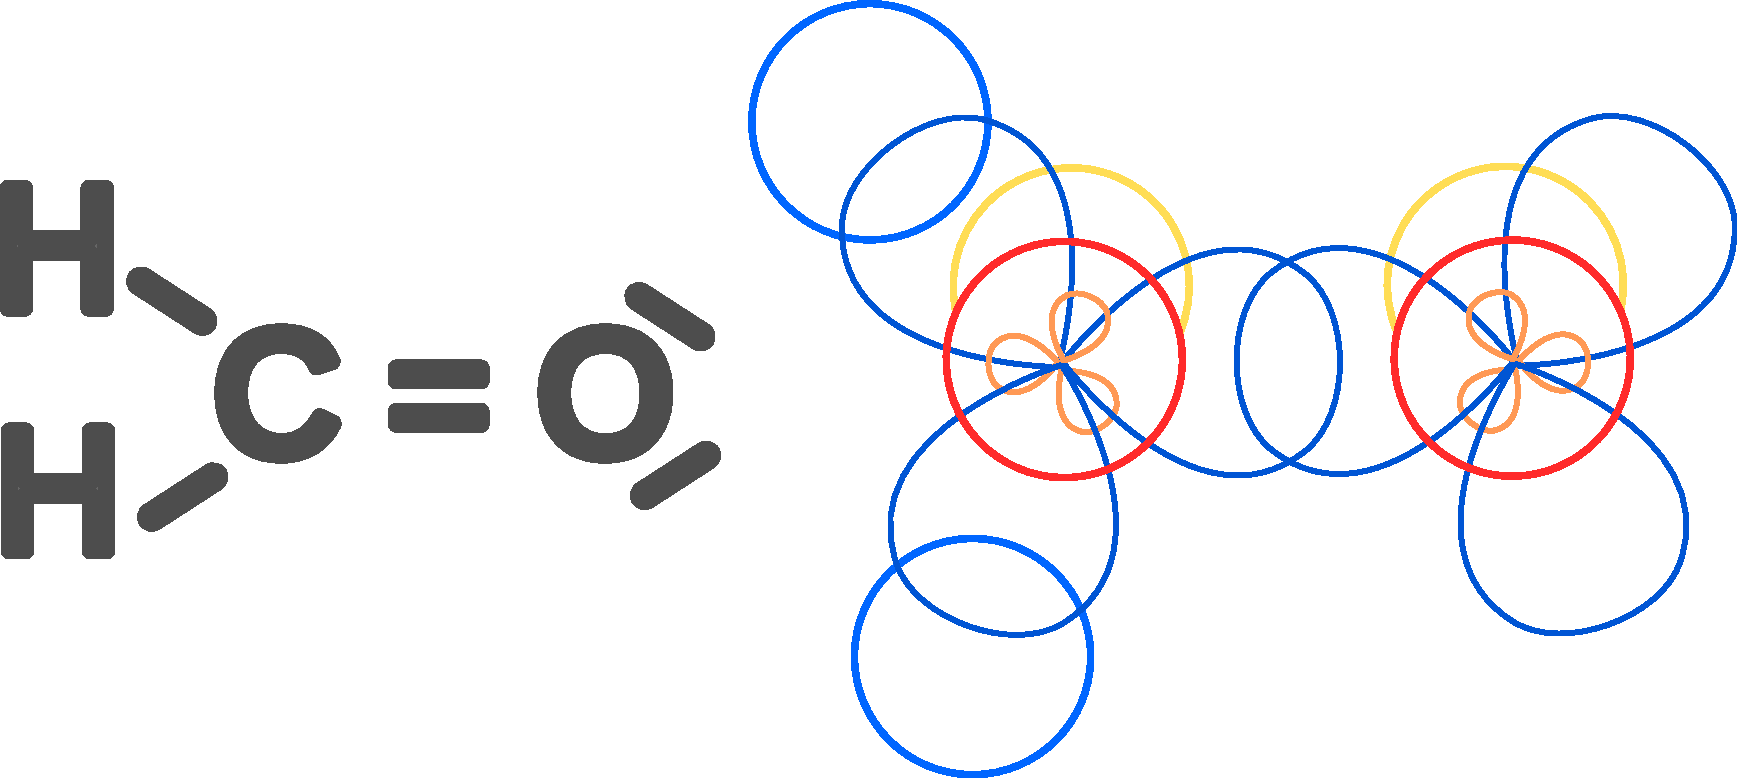
\includegraphics[scale=0.3]{representation_OA}

Ici, les OA blues forment le système $\sigma$ et celles en rouge le système $\pi$.
\subsection{Exceptions}
Parfois les hybridations choisies ne sont pas compatibles avec d'autres formes mésomère ``secondaires'' de la molécules. Il faut alors souvent baisser le niveau d'hybridation pour ajouter une OA non hybridée et ainsi créer une liaison $\pi$, seule à pouvoir \^etre délocalisée.

On peut représenter les OA de la molécule d'HCOOH :

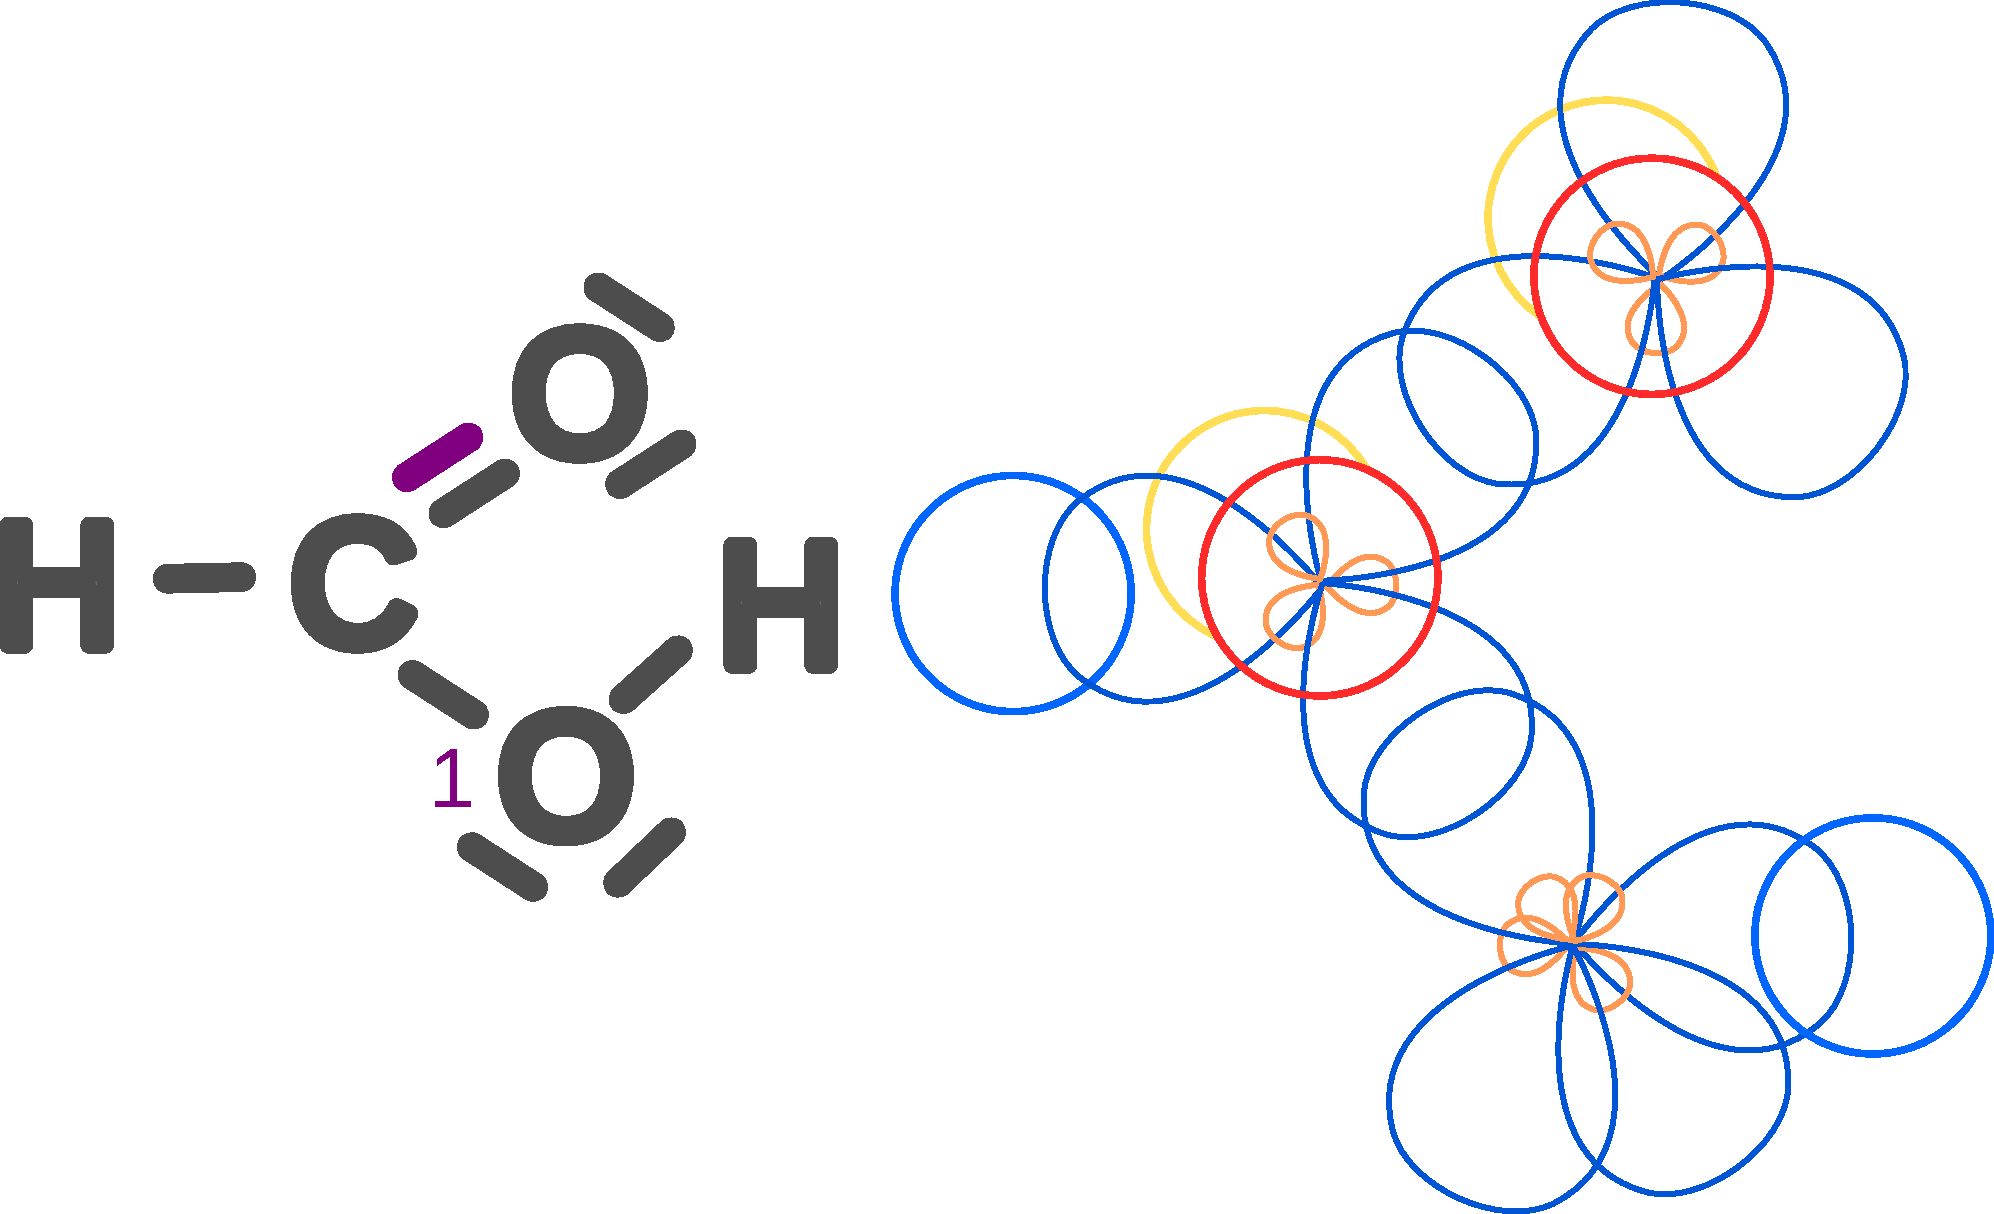
\includegraphics[scale=0.25]{form_1}

Cependant, une forme mésomère existe. Il y a donc délocalisation de la liaison violette. Or, sur le schéma précédant, l'Oxygène 1 n'a pas d'OA non hybridée pouvant réaliser une liaison $\pi$. Il faut donc baisser le degré d'hybrdidation\marginTips{Souvent, il faudra simplement passer de $sp^3$ à $sp^2$.} pour cet atome, comme sur le schéma ci-dessous, qui est la bonne représentation, respectant les 2 formes mésomères :

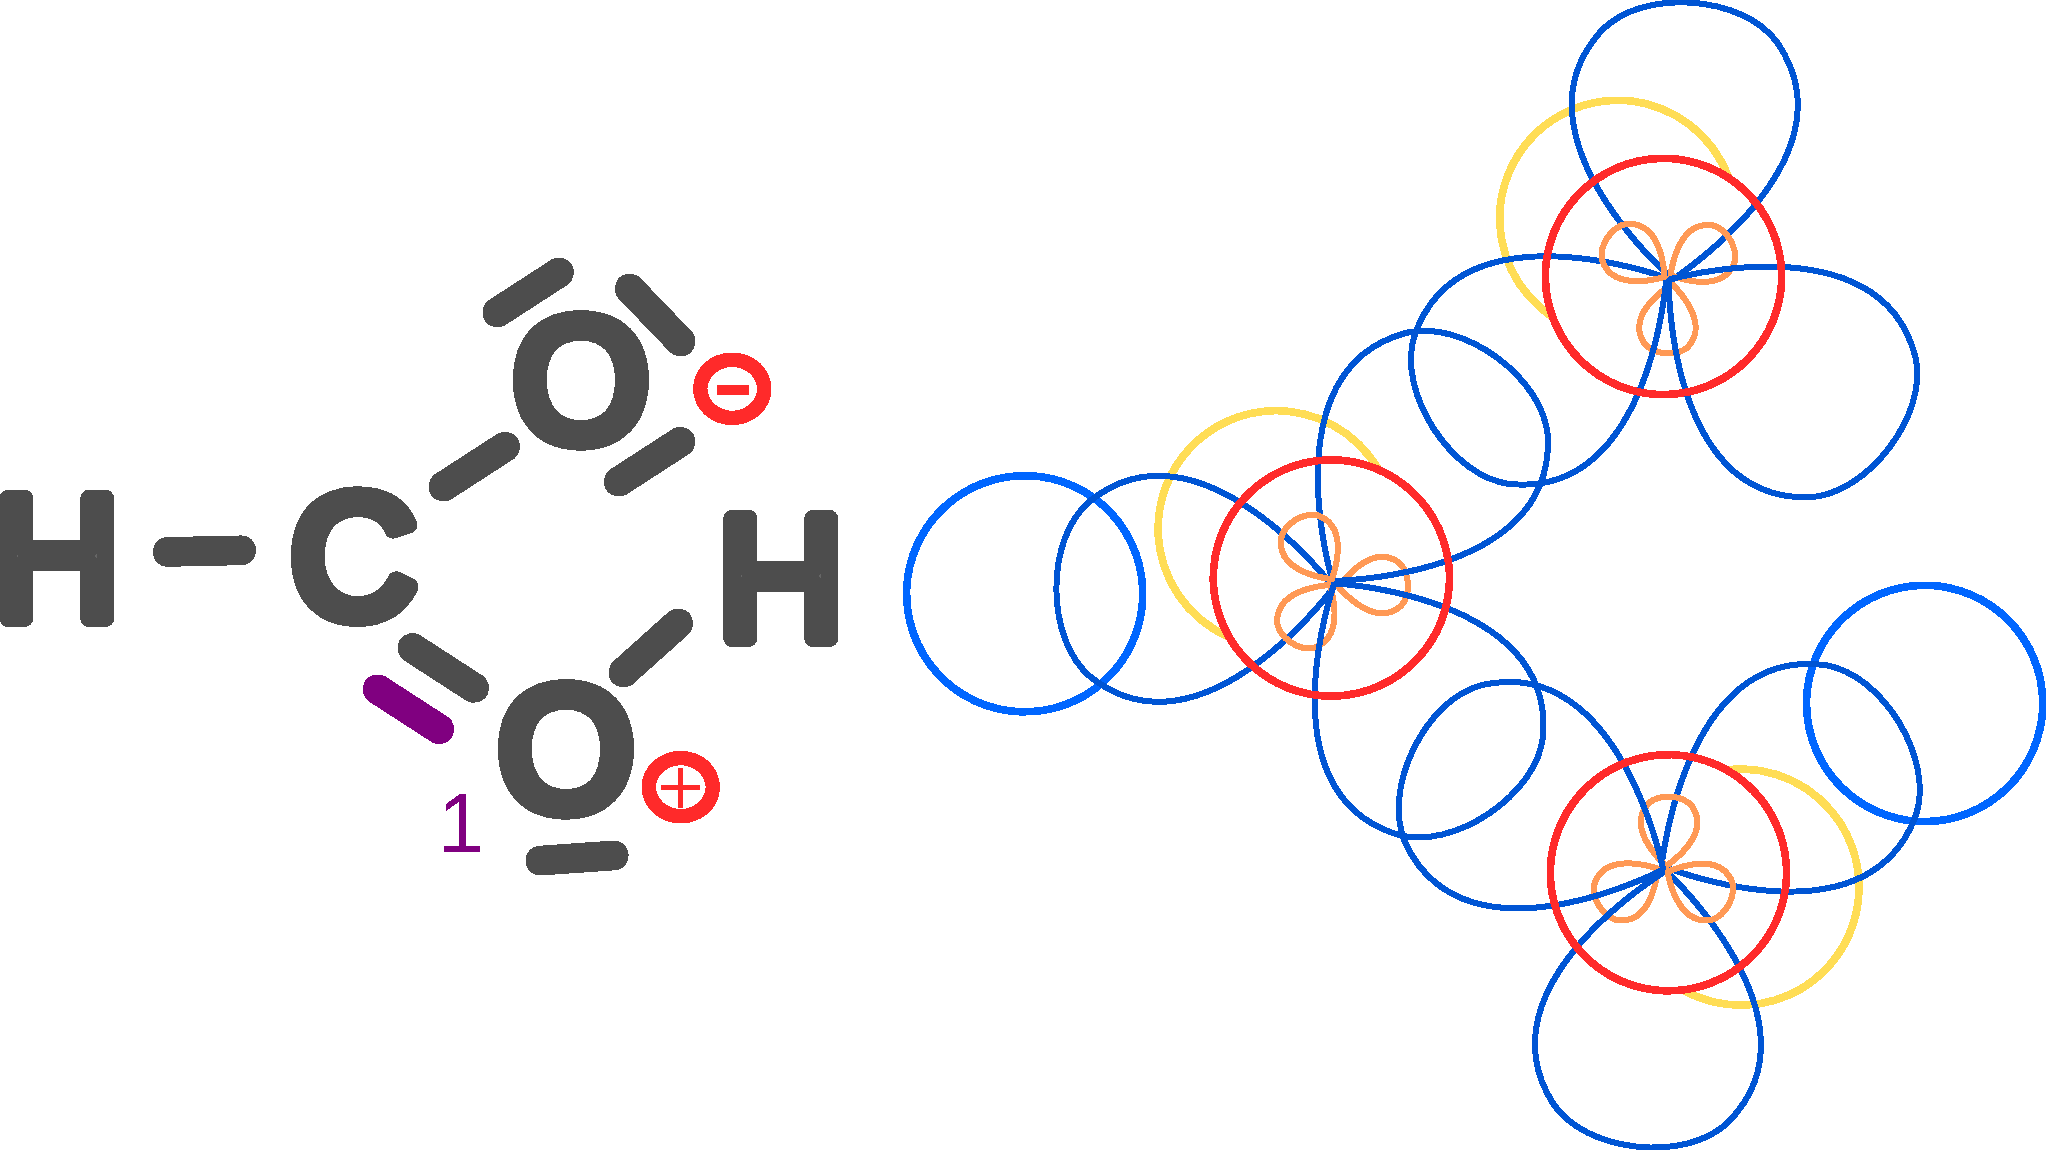
\includegraphics[scale=0.25]{form_2}
\subsection{Remarques}
\subsubsection{Hybridation}
Seuls les électrons $\pi$ \emph{dans le m\^eme plan} peuvent se délocaliser. Dans l'exemple ci-dessous, seuls les électrons des OA rouges peuvent se délocaliser car dans le m\^eme plan. Les vertes sont dans leur propre plan et n'ont pas de possibilité de délocalisation.

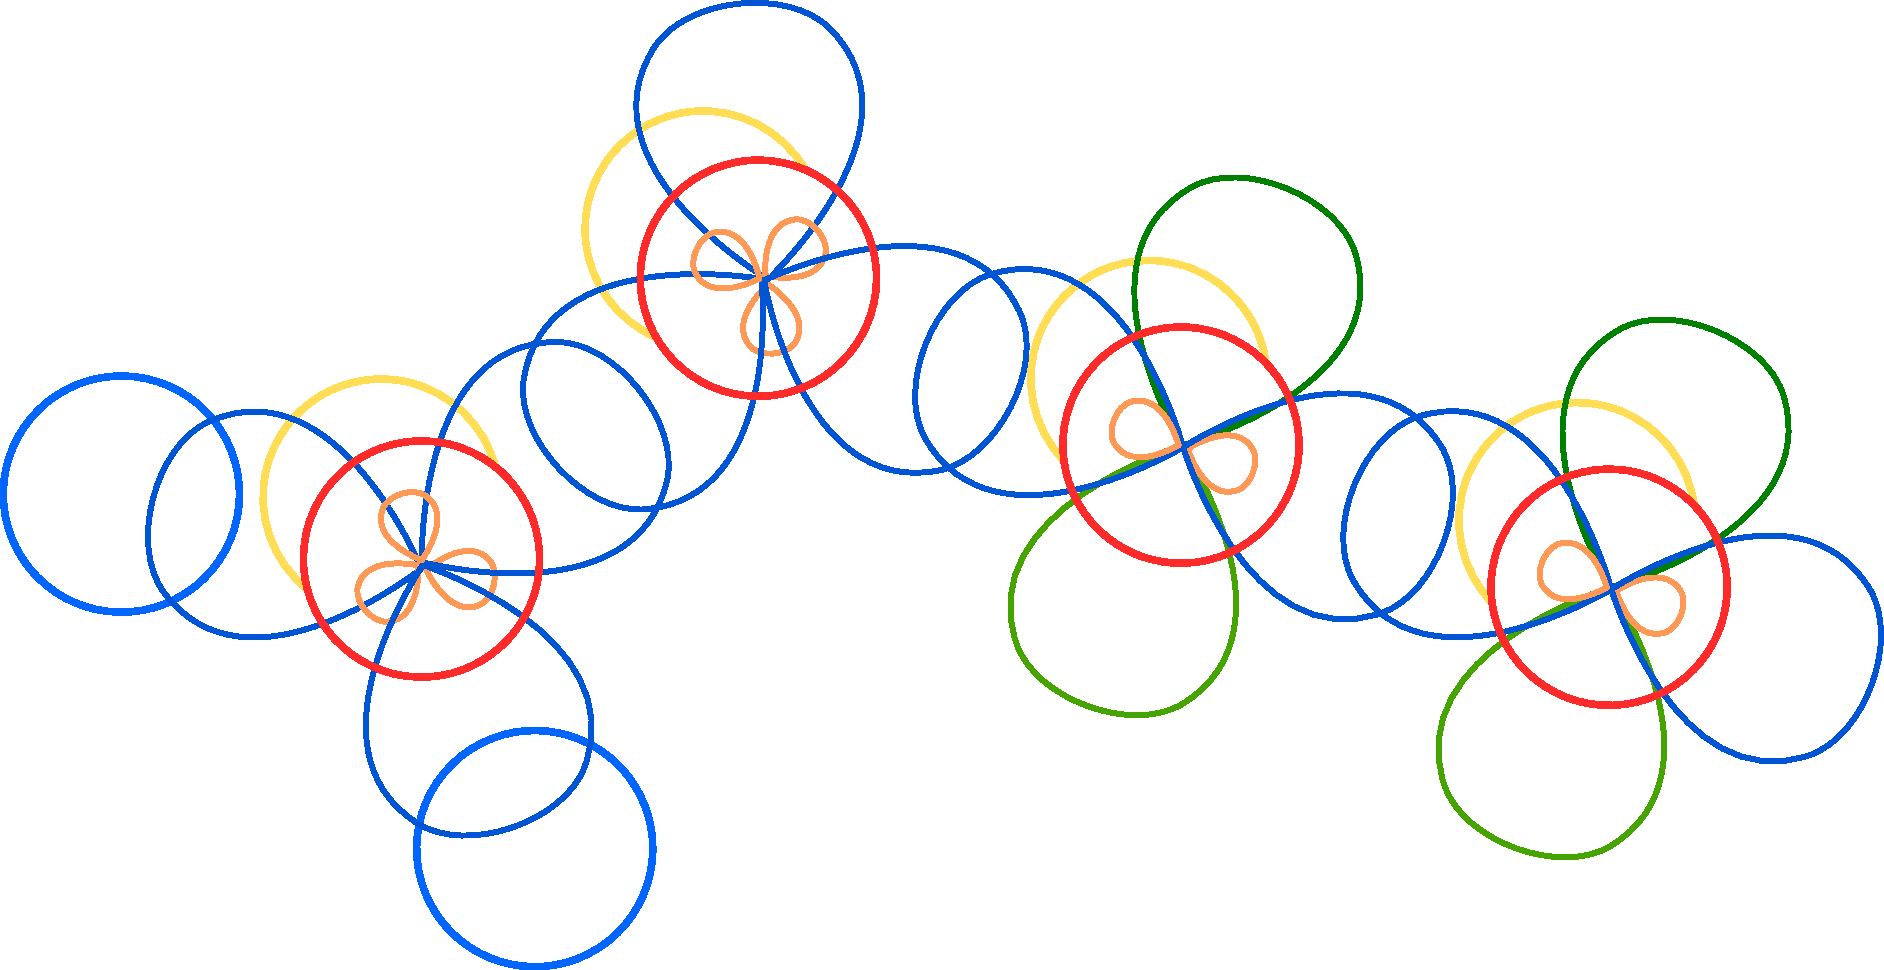
\includegraphics[scale=0.3]{s1}

Pour compter le nombre d'électrons participant au système $\pi$ dans le cas d'une délocalisation, il faut compter le nombre de Doublets qui se déplacent pour former les formes mésomères et diviser par 2.\marginCritical{Il se peut qu'il y ait plus d'électrons que d'OA non hybridées, car une OA peut décrire 2 électrons. C'est le cas pour un DNL participant au système : il sera décrit par une seule OA non hybridée mais comptera pour 2 électrons.}
\subsubsection{Hybride de résonance}
L'hybride de résonance d'une molécule est le mélange entre les formes mésomères où toutes les doubles liaisons possibles des 2 formes sont représentées avec des pointillés.
\subsubsection{Forme mésomère}
Dans la plupart des cas, pour qu'une forme mésomère soit prise en compte, il faut que les atomes mis en jeu respectent quand m\^eme la règle de l'octet.\marginCheck{Cependant, il peut arriver que des formes issues d'une délocalisation $\pi$ ne respectent pas les règles.}


% \section{Diagrammes d'OA moléculaires}
% \subsection{Introduction}
% Il vaut $S = \int\int\int \psi_{n,l,m}\psi_{n'l',m'} \mathrm{d}\tau$. Le signe n'est pas important. Si c'est non nul, il y a une intéraction, donc une liaison.
%
% On fait une approximation : $\psi = \prod^{10}_{i=1} \varphi_i(x_i,y_i,z_i)$. $\varphi$ est appelé orbitale moléculaire.
%
% On fait l'approximation LCAO avec une combinaison linéaire des OA : $\varphi_i = c_1\chi_1 + c_2\chi_2+\dots = \sum_k c_k\chi_i$.\marginInfo{On les exprime comme une combinaison linéaire d'OA}
%
% La combinaison linéaire de $n$ OA génère $n$ OM. Pour 2 OA, on fait une somme ou une différence.
% \subsection{Recouvrement}
% Schéma 2
% Avec 2  OA $s$, le produit de 2 fonctions + est non nul.
% Avec
%
% \begin{theorem}[Recouvrement]
% 2 OA avec des symétries différentes par rapport à un plan contenant la liaison ont des recouvrement nuls
% \end{theorem}
% \subsection{Types d'OM}
% La combinaison génère presque toujours\marginInfo{Sauf si les 2 OA ont un recouvrement nul. Dans ce l'OM est les 2 OA de départs} :
% \begin{itemize}
%  \item Une OM liante
%  \item Une OM anti-liante
% \end{itemize}
% Cela dépend du signe de recouvrement (les OA sont définies au signe près). C'est un choix que l'on fait selon le signe de départ. On a toujours une liante et une non liante cependant.
% \subsection{Énergie}
% Schema 3
% \subsection{Ordre de liaison}
% \[p = \frac{Nb(eLiant)-Nb(eAntiLiante)}{2}\]
%
% Pour le DOM précédant : \[p = \frac{2-0}{2} = 1\]. Quand l'ordre de liaison correspond à ce qu'on a sur un schéma de Lewis, Lewis foncionne bien pour cette molécule.
% \subsection{Constrution}
% Gros et en couleurs.
\section{Orbitales moléculaires}
\subsection{Approximations}
\subsubsection{Approximation orbitale}
Cette première approximation est utilisée en raison de l'impossibilité qu'il y a à trouver une solution analytique exacte pour la fonction d'onde dès que le système étudié possède plus d'un électron. Une solution est donc d'écrire la fonction d'onde polyélectronique dépendant des coordonnées de $n$ électrons comme le produit de fonctions monoélectroniques dépendant  des coordonnées d'un seul électron :
\begin{equation}
 \theta_{el} = \varphi_1(e_1)\varphi_2(e_2)\dots\varphi_n(e_n)
\end{equation}
\warningInfo{OM}{Ces fonctions $\varphi_i$ sont appellées Orbitales Moléculaires du système considéré.}
\subsubsection{Théorie LCAO}
Reste encore à choisir la forme pour chaque OM. La solution la plus simple est d'écrire chaque OM comme une combinaison linéaire des OA des atomes constituants les atomes. On obtient, avec $c$ les coefficients et $\chi$ les OA\marginCritical{Les orbitales décrivant les électrons de coeur ne sont pas prises en compte} :
\begin{equation}
\varphi_i = \sum_j c_{i,j}\chi_j
\end{equation}
\subsection{Recouvrement}
Le recouvrement désigne la surface dans laquelle les 2 OA générées à partir de la combinaison intéragissent. Le plus important est de déterminer s'il est nul ou non.
\begin{theorem}[Recouvrement]
2 OA avec des symétries différentes par rapport à un plan  ont des recouvrement nuls
\end{theorem}
Pour déterminer le signe du recouvrement, on fait le produit des cotés des OA les plus proches du centre.

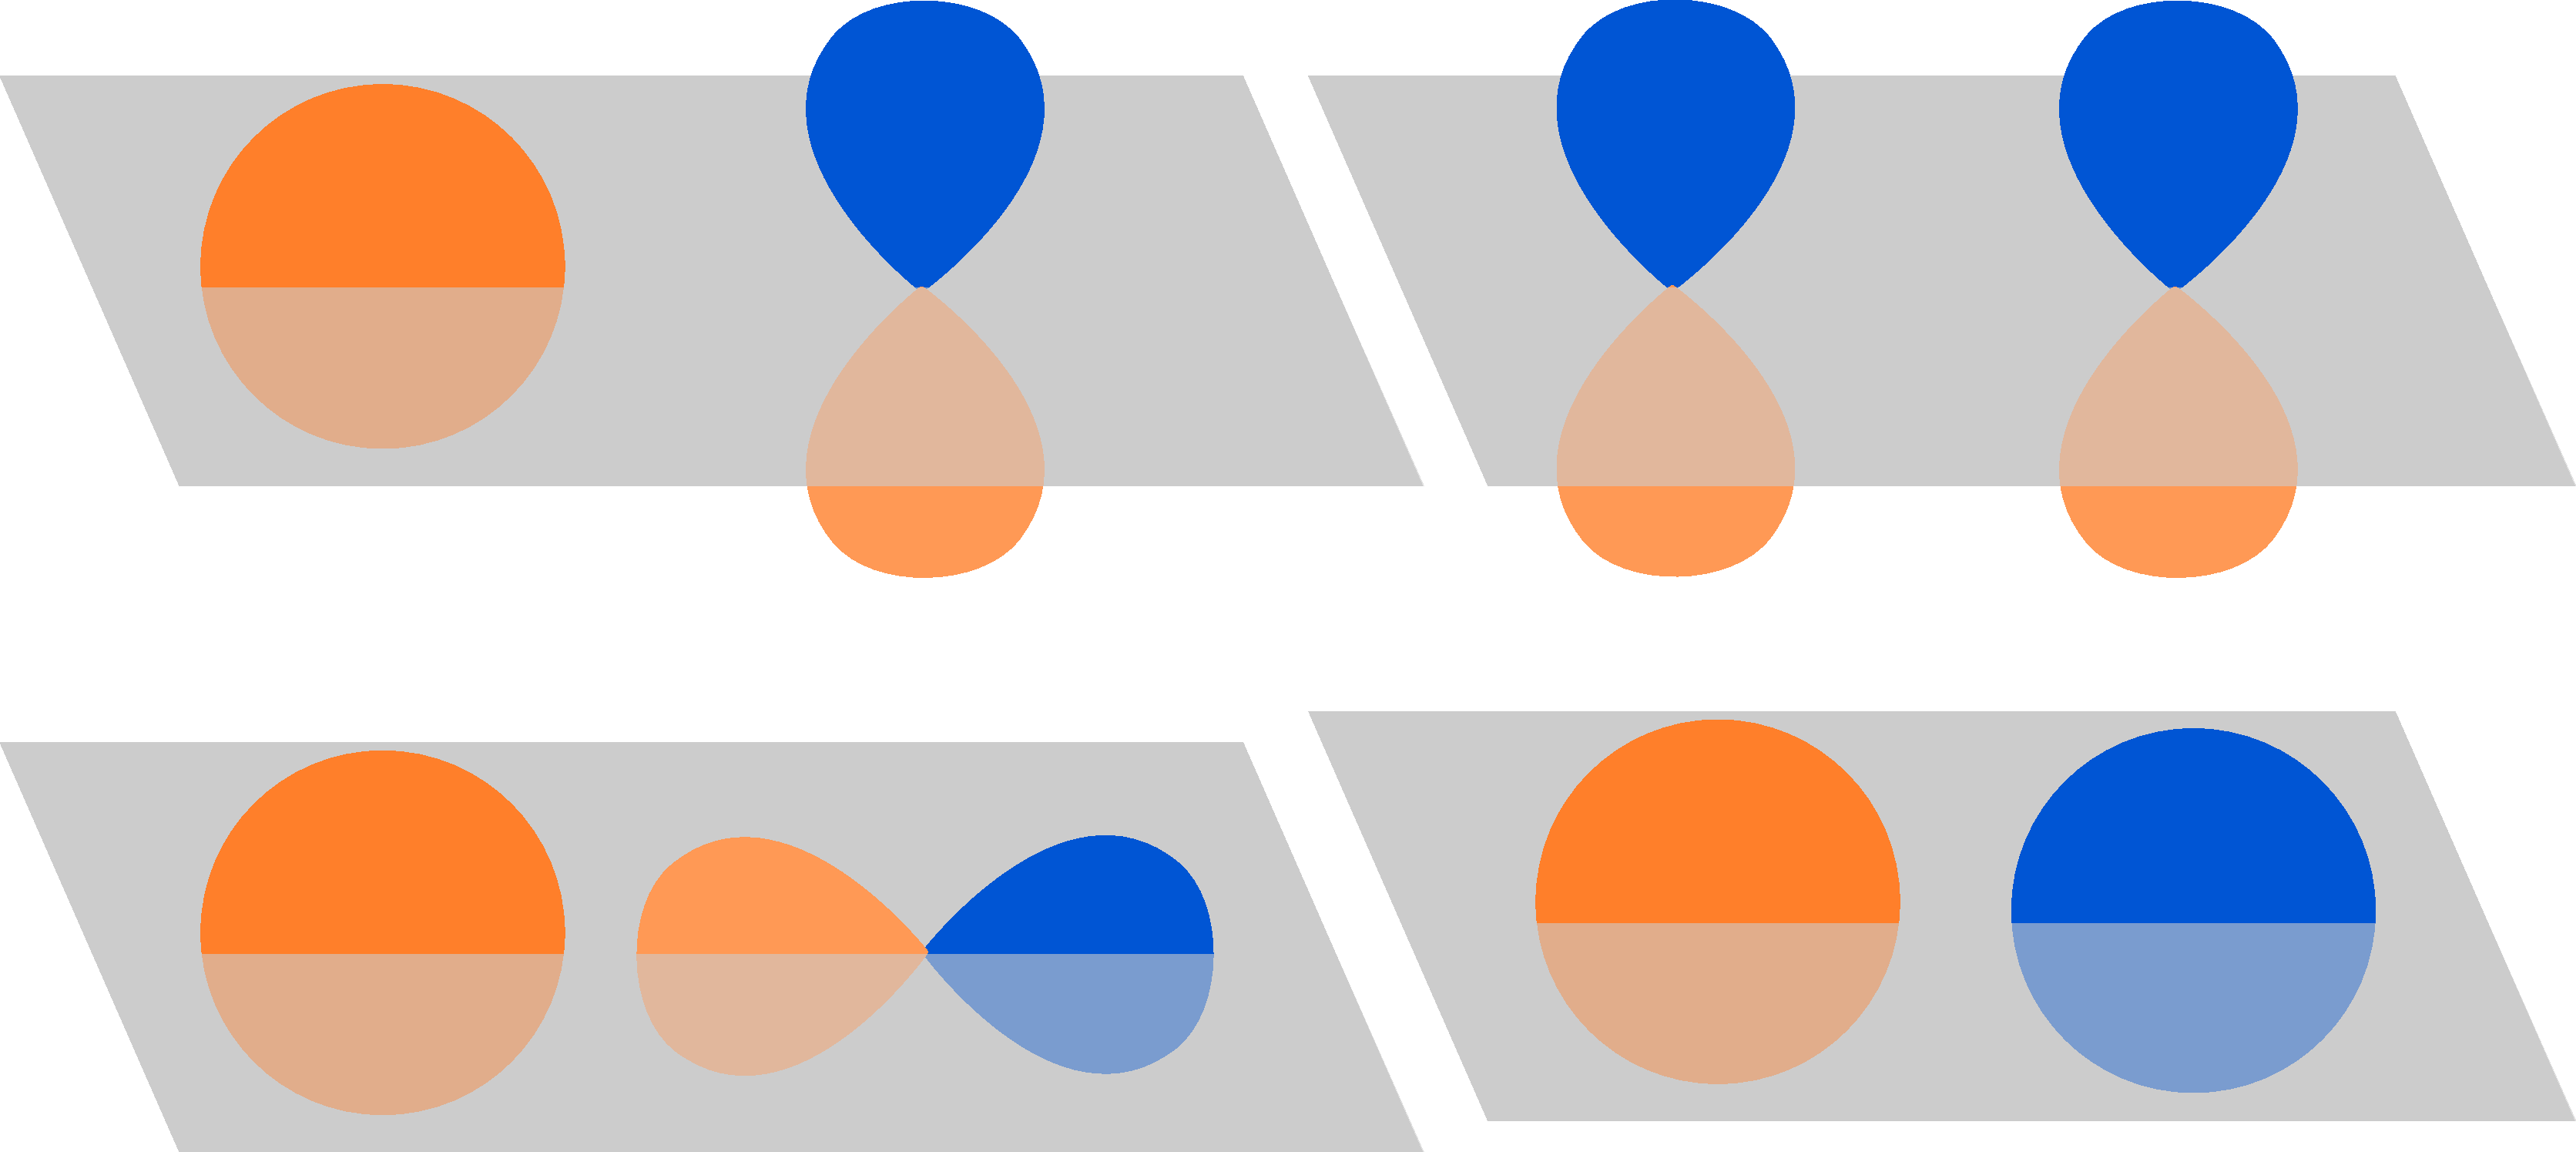
\includegraphics[scale=0.1]{recouvrement}

Sur l'exemple, la première a un recouvrement nul, la deuxième et troisème un positif et la dernière un négatif.
\subsection{Types d'OM}
La combinaison génère presque toujours\marginInfo{Sauf si les 2 OA ont un recouvrement nul. Dans ce cas l'OM est les 2 OA de départs} :
\begin{itemize}
 \item Une OM liante
 \item Une OM anti-liante
\end{itemize}
Cela dépend du signe de recouvrement (les OA sont définies au signe près). C'est un choix que l'on fait selon le signe de départ. On a toujours une liante et une non liante cependant.
\subsection{Construction du DOM}
On place toujours l'OM anti-liante en haut car c'est la plus haute en énergie. Pour l'indiquer, on note $\sigma *$. On peut mettre des pointillés si les OA sont très éloignées en énergie des OM. De plus, on indique où se trouve les électrons.

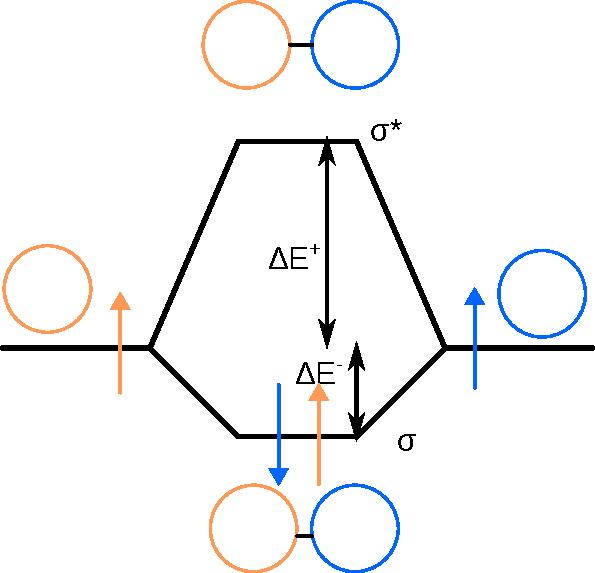
\includegraphics[scale=0.5]{s00}
\subsection{Ordre de liaison}
\[p = \frac{Nb(eLiant)-Nb(eAntiLiante)}{2}\]

Pour le DOM précédant : \[p = \frac{2-0}{2} = 1\] Quand l'ordre de liaison correspond à ce qu'on a sur un schéma de Lewis, cela signifie que Lewis fonctionne bien pour cette molécule.
\subsection{Force d'interaction}
Elle dépend de la surface de contact et de la différence d'énergie : $\Delta E^+ = \frac{S^2}{E_1-E_2}$. Si le rapport est supérieur à 15eV, on néglige l'intéraction entre les 2 OA.
\subsection{Liaison ionique}
Lorsque la différence de niveaux d'énergie entre orbitales atomiques de deux atomes est suffisamment élevée, les orbitales de l'un des atomes contribuent presque entièrement aux OM liantes, et les orbitales de l'autre atome contribuent presque entièrement aux OM anti-liantes. Dans ce cas, un ou plusieurs électrons sont transférés d'un atome à l'autre, ce qui donne une liaison ionique.
\end{document}

